\documentclass[a4paper,12pt,oneside]{article}

\frenchspacing

\usepackage[utf8]{inputenc}
\usepackage{t1enc}
\usepackage{amsmath}
\usepackage{amssymb}
\usepackage{t1enc}
\usepackage{ae}
\usepackage{subfigure}
\usepackage[font=small,labelfont=bf,up,textfont=it,up]{caption}
\usepackage{color}
\usepackage{array}
\usepackage{longtable}
\usepackage{calc}
\usepackage{multirow}
\usepackage{hhline}
\usepackage{ifthen}
\usepackage{amssymb}
\usepackage{bm}
\usepackage{ifpdf}
\ifpdf
	\usepackage[pdftex]{graphicx}
	\usepackage[pdftex]{hyperref} 
	\hypersetup{colorlinks=true,
		pdfstartview=FitV,
		linkcolor=blue,
		citecolor=red,
		urlcolor=blue,
		pdfauthor={HORVATH Laszlo, horla@reak.bme.hu},
		pdfsubject={},
		pdftitle={Short Time Fourier Transform in NTI Wavelet Tools}}
	\DeclareGraphicsExtensions{.pdf}
\else
	\usepackage{graphicx}
	\usepackage{epsfig}
	\DeclareGraphicsExtensions{.eps}
	\newcommand{\url}[1]{#1}
\fi

\usepackage[sort&compress]{natbib}

\def\inputGnumericTable{}
\graphicspath{{figs/}}

\pagestyle{plain}

\definecolor{fgreen}{RGB}{0,161,75}
\definecolor{szurke}{RGB}{100,100,100}
\definecolor{myblue}{RGB}{0,174,239}

\newcommand{\dt}{\mathrm{d}t}
\newcommand{\df}{\mathrm{d}f}
\newcommand{\du}{\mathrm{d}u}
\newcommand{\dxi}{\mathrm{d}\xi}
\newcommand{\dw}{\mathrm{d}\omega}
\newcommand{\conj}{^{\textstyle^*}}
\newcommand{\Abs}{\mathrm{A}}
\newcommand{\Arg}{\Phi}
\newcommand{\R}{\mathrm{R}}
\newcommand{\I}{\mathrm{I}}


\title{\textbf{Short Time Fourier Transform\\in NTI Wavelet Tools}}

\author{
Written by László Horváth$^1$ \vspace{0.3 cm}\\
Supervisors:\\
Dr. Gergő I. Pokol$^1$, Dr. Marco Sertoli$^2$, Gergely Papp$^1$ \vspace{0.3 cm}\\ 
{\footnotesize $^1$Institute of Nuclear Techniques, Budapest University of Technology and Economics,}\vspace{-0.2 cm}\\
{\footnotesize EURATOM Association, Pf 91, H-1521 Budapest, Hungary
}\\
{\footnotesize $^2$Max-Planck-Institut für Plasmaphysik,}\vspace{-0.2 cm}\\
{\footnotesize EURATOM Association, D-85748 Garching, Germany}\\
{\footnotesize E-mail: horla@reak.bme.hu}}

\begin{document}

\maketitle

\clearpage
\tableofcontents

%\vspace{2 cm}
%\noindent
%\emph{All of the figures presented in this report were produced by the \emph{\textbf{NTI Wavelet Tools 1.2.0}} program, available at the IPP via MTR.}

\thispagestyle{empty}
\newpage

\section{Introduction}

NTI Wavelet Tools\cite{nti12} is a data processing toolbox that is developed and maintained by the Institute of Nuclear Techniques (NTI), Budapest University of Technology and Economics. The current development language is IDL\cite{idl12} (Interactive Data Language). The toolbox features a graphical user interface (GUI) with a collection of tools based on continuous time-frequency transforms - ideal for processing transient signals - and incorporates various other data processing methods that can be run from command line.

\section{Linear time-frequency transformations}

The forthcoming summary is based on the work of Mallat\cite{mallat08wavelet}. Linear time-frequency transformations can be calculated by correlating the signal with families of so-called time-frequency atoms:
\begin{equation}\label{eq:transform}
  T f(u,\xi) = \langle f, g_{u, \xi} \rangle = \int\limits_{-\infty}^{+\infty} f(t) g^*_{u, \xi}(t) \dt\ ,
\end{equation}
where $g_{u, \xi}$ is a time-frequency atom, a complex function. $u$ and $\xi$ are the time and frequency indices of the atom identifying its position on the time-frequency plane and the $*$ represents the complex conjugation. The energy of a time-frequency atom is well localized in both time and frequency, and
\begin{equation}
  \| g_{u, \xi}(t) \|^2 = \langle g,g \rangle = \int\limits_{-\infty}^{+\infty} |g(t)|^2 \dt = 1 \ .
\end{equation}

The center of the atom in time ($u$) and in frequency ($\xi$) can be defined as
	\begin{equation*}
	u = \int\limits_{-\infty}^{+\infty} t \cdot |g_{u, \xi}(t)|^2 \dt\ ,
	\end{equation*}
	\begin{equation*}
	\xi = \frac{1}{2\pi} \int\limits_{-\infty}^{+\infty} \omega \cdot |G_{u, \xi}(\omega)|^2 \dw\ .
	\end{equation*}
The extent of the atom in time ($\sigma_t$) and in frequency ($\sigma_{\omega}$) can be defined in the following way:
	\begin{equation*}
	\sigma_t^2 = \int\limits_{-\infty}^{+\infty} (t-u)^2 \cdot |g_{u, \xi}(t)|^2 \dt\ ,
	\end{equation*}
	\begin{equation*}
	\sigma_{\omega}^2 = \frac{1}{2\pi} \int\limits_{-\infty}^{+\infty} (\omega-\xi)^2 \cdot |G_{u, \xi}(\omega)|^2 \dw\ ,
	\end{equation*}
where $G$ denotes the Fourier-transform of $g$.

The energy density can then be calculated by taking the absolute value squared \cite{mallat08wavelet}:
\begin{equation}\label{eq:energy_density}
  E f(u,\xi) = |T f(u,\xi)|^2\ .
\end{equation}
The energy density calculated from STFT is called spectrogram.

\subsection{Short time Fourier transform}

One choice in NTI Wavelet Tools to investigate transient signals is using short time Fourier transform\cite{mallat08wavelet} (STFT), which is a continuous time-frequency transform. The time-frequency atoms of STFT are generated by shifting an atom in time and frequency:
\begin{equation}\label{eq:stft-atom}
  g_{u,\xi}(t) = e^{i\xi t} g(t-u) \ .
\end{equation}
Therefore STFT takes the following form:
\begin{equation}\label{eq:stft}
  S f(u,\xi) = \langle f, g_{u, \xi} \rangle = \int\limits_{-\infty}^{+\infty} f(t) e^{-i \xi t} g(t-u) \dt \ ,
\end{equation}
where $g(t-u)$ is a real function. NTI Wavelet Tools uses Gabor-atoms, i.e. a Gaussian-window for $g(t)$ in \eqref{eq:stft-atom}.

\section{Energy in signal processing}

In signal processing the energy of an $f(t)$ time signal, where $t\in[0,T]$ can be defined in the following way:
\begin{equation}\label{eq:energy}
  E = \int\limits_0^T |f(t)|^2 \dt \ .
\end{equation}

\subsection{Energy and amplitude}

The \eqref{eq:energy_density} energy density gives the energy carried by the wave, per unit time and frequency. It is also expected to get the amplitude of the signal components, therefore we have to calculate the energy of a harmonic wave, i.e. a cosine function. Let
\begin{equation}\label{eq:cos}
  f(t) = A \cdot \cos(\omega_0 t) \quad t \in[0, T] \ .
\end{equation}
The energy of \eqref{eq:cos} is
\begin{eqnarray}\label{eq:cos_energy}
  & E = \int\limits_0^T |f(t)|^2 \dt = \int\limits_0^T |A \cdot \cos(\omega_0 t)|^2 \dt = \nonumber\\
  & = A^2 \int\limits_0^T \cos^2(\omega_0 t) \dt = A^2 \int\limits_0^T \dfrac{1 + \cos(2\omega_0 t)}{2} \dt
\end{eqnarray}
\begin{equation}\label{eq:cos_energy2}
  E = A^2 \left[\dfrac{t}{2}\right]_0^T + A^2 \left[\dfrac{\sin(2\omega_0 t)}{4\omega_0}\right]_0^T\ , 
\end{equation}
\begin{equation}\label{eq:cos_energy3}
  E \approx \dfrac{A^2 T}{2} \ ,
\end{equation}
in the case if $T = n\cdot \dfrac{\pi}{2\omega_0}$, where $n \in \mathbb{Z}$. If $T \neq n\cdot \frac{\pi}{2\omega_0}$ the ratio of the second and the first term in equation \eqref{eq:cos_energy2} tends to $0$, as $T$ tends to infinity, since the value of the second term is between $-\frac{A^2}{4 \omega_0}$ and $+\frac{A^2}{4 \omega_0}$.

Equation \eqref{eq:cos_energy} means that, if one knows the energy carried by the wave, the amplitude can be evaluated by
\begin{equation}\label{eq:amplitude}
  A = \sqrt{\dfrac{2 E}{T}} \ .
\end{equation}

\subsection{Energy density on the time-frequency plane}

The energy density calculated from STFT by equation \eqref{eq:energy_density} contains also the energy carried by the negative frequencies. NTI Wavelet Tools has been developed to investigate real signals, so the results belonging to the negative frequencies do not provide additional information about the signal since
\begin{equation}\label{negative_freq}
  S f(u,\xi) = S\conj f(u,-\xi) \ .
\end{equation}
However if one wants to compare the energy provided by the spectrogram and the energy of a cosine function, the negative frequencies must be taken into account. Because STFT does not divide the signal into cosine functions, but into $e^{-i \omega t}$ functions with different frequencies. A cosine function will be modelled as:
\begin{equation}\label{eq:cosine}
  \cos(\omega t) = \dfrac{e^{i\omega t} + e^{-i\omega t}}{2} \ ,
\end{equation}
and the energy of a cosine function will be divided in both positive and negative frequencies. NTI Wavelet Tools plots only the positive frequencies of the energy density, but it is multiplied by 2 so to satisfy Parseval's theorem:
\begin{equation}\label{eq:parseval}
  \int\limits_{-\infty}^{+\infty}  |T f(u,\xi)|^2 \du \dxi = \int\limits_{-\infty}^{+\infty}  |f(t)|^2 \dt \ .
\end{equation}
In this way the energy of the signal on a $[u_1, u_2]$ time interval and a $[\xi_1, \xi_2]$ frequency interval can be evaluated by
\begin{equation}\label{eq:energy_interval}
  E_{u_1, u_2, \xi_1, \xi_2} = \int\limits_{\xi_1}^{\xi_2} \int\limits_{u_1}^{u_2} |T f(u,\xi)|^2 \du \dxi \ ,
\end{equation}
and the unit of the energy density will be\footnote{e.g.: if the physical unit of the measured signal was $[\mathrm{eV}]$, the unit of the energy density would be $[\mathrm{eV}^2 \cdot \mathrm{s}]$.}
$$\dfrac{[\mathrm{Signal\ Energy}]}{\mathrm{s}\cdot\mathrm{Hz}} = [\mathrm{Signal\ Energy}] = [\mathrm{Signal}]^2\cdot \mathrm{s} \ ,$$ where the energy is defined as in \eqref{eq:energy}.

To avoid the problems caused by the zero frequency, it is convenient to subtract the mean of the signal from it before starting the analysis\footnote{NTI Wavelet Tools starts processing with subtracting the mean value of the signal.}.

\subsection{Wave amplitude determination from energy density}

In some cases, it is expected to calculate the amplitude of the signal components from the spectrogram. Since the time-frequency resolution of the transform cannot be arbitrarily fine, the energy of a signal component will be spread on the time-frequency plane. If the investigated signal consists of harmonic components and the frequency resolution is sufficiently good to separate them, the signal energy can be evaluated by integrating the energy density on the required bandwidth and time interval using equation \eqref{eq:energy_interval}. Considering equation \eqref{eq:amplitude} the amplitude will be:
\begin{equation}\label{eq:amplitude2}
  A = \sqrt{\frac{2E}{T}} = \sqrt{\frac{2E_{u_1, u_2, \xi_1, \xi_2}}{u_2-u_1}} \ .
\end{equation}
The required frequency bandwidth can be determined from the properties of the used time-frequency atoms. The Gabor-atom takes the following form:
\begin{equation}\label{eq:gt}
  g(t) = \frac{1}{\sqrt{\sqrt{2\pi}\sigma_t}} \cdot \exp\left\{-\frac{(t-u)^2}{2\sigma_t^2}\right\} \ .
\end{equation}
In order to get the width of the atom on the frequency plane, one has to calculate the Fourier-transform of the term in equation \eqref{eq:gt}. Since the $u$ time shift affects only the phase of transformed atom, but not the width, it is convenient to carry out the transform in case of $u=0$:
\begin{eqnarray}\label{eq:fgt}
  & G(\omega) = \int\limits_{-\infty}^{+\infty} g(t) e^{-i\omega t} \dt = \nonumber\\
  & = \int\limits_{-\infty}^{+\infty} \dfrac{1}{\sqrt{\sqrt{2\pi}\sigma_t}} \cdot \exp\left\{-\dfrac{t^2}{2\sigma_t^2}\right\} \left( \cos(\omega t) - i\sin(\omega t) \right) \dt  = \nonumber\\
  & = \dfrac{1}{\sqrt{\sqrt{2\pi}\sigma_t}} \int\limits_{-\infty}^{+\infty} \exp\left\{-\dfrac{t^2}{2\sigma_t^2}\right\} \cos\left(2 \cdot \dfrac{\omega}{2} \cdot  t \right) \dt + \nonumber\\
  & + \dfrac{-i}{\sqrt{\sqrt{2\pi}\sigma_t}} \int\limits_{-\infty}^{+\infty} \exp\left\{-\dfrac{t^2}{2\sigma_t^2}\right\} \sin(\omega \cdot  t) \dt \ .
\end{eqnarray}
The second integrand is odd, so integration over a symmetrical range is equal to 0. Since \cite{bronshtein07handbook}:
\begin{equation}\label{eq:first_int}
  \int\limits_{-\infty}^{+\infty} e^{-at^2} \cos(2xt) \dt = \sqrt{\dfrac{\pi}{a}} \cdot e^{\frac{x^2}{a}} \ ,
\end{equation}
equation \eqref{eq:fgt} can be re-written as:
\begin{eqnarray}\label{eq:second_int}
  & G(\omega) = \dfrac{1}{\sqrt{\sqrt{2\pi}\sigma_t}} \cdot \sqrt(2 \pi) \cdot \sigma_t \cdot \exp\left\{-\dfrac{\omega^2 \sigma_t^2}{2}\right\}  = \nonumber\\
  & = \sqrt{\sqrt{2\pi}\sigma_t} \cdot \exp\left\{-\dfrac{\omega^2}{2 \cdot \left( \dfrac{1}{\sigma_t} \right)^2}\right\} \ .
\end{eqnarray}
The extent of the atom in frequency\footnote{$f = \frac{\omega}{2\pi}$} is therefore:
\begin{equation}\label{eq:extent}
  \sigma_{f} = \dfrac{\sigma_{\omega}}{2 \pi} = \dfrac{1}{2 \pi \sigma_{t}} \ .
\end{equation}

\subsubsection{Evaluate amplitude by integral}

Integrating a Gaussian function over $6 \cdot \sigma$ interval would contain the $99.6 \%$ of its energy. However the $\sigma_{f}$ calculated in \eqref{eq:extent} is the extent of the window in the STFT, but not in the energy density:
\begin{equation}\label{eq:extent_energy}
  \Bigg( a \cdot \exp\left( \frac{x^2}{2\sigma_{\textrm{STFT}}^2} \right) \Bigg)^2 = 
  a^2 \cdot \exp\left( \frac{x^2}{2 \left( \dfrac{\sigma_{\textrm{STFT}}}{\sqrt{2}} \right)^2} \right) =
  a^2 \cdot \exp\left( \frac{x^2}{2 \sigma_{\textrm{ED}}^2} \right) \ ,
\end{equation}
\begin{equation}\label{eq:extent_energy_stft}
  \sigma_{\textrm{ED}} = \dfrac{\sigma_{\textrm{STFT}}}{\sqrt{2}}  = \dfrac{\sigma_f}{\sqrt{2}} \ .
\end{equation}
So to integrate over $6 \cdot \sigma$ interval in the energy density to get the wave energy one has to use $\sigma_{\textrm{ED}}$ defined in \eqref{eq:extent_energy_stft}.

\subsubsection{Evaluate amplitude from peak energy}

An other method is taking the maximum value of the energy density in the required bandwidth and calculate the wave energy analytically:
\begin{equation}\label{eq:energy_analytical}
  \int\limits_{-\infty}^{+\infty} \Bigg( a \cdot \exp\left( \frac{x^2}{2\sigma_f^2} \right) \Bigg)^2 \dt = 
  a^2 \cdot \sigma_f \cdot \sqrt{\pi} \ .
\end{equation}
Therefore if the peak of the energy density is $E_{\textrm{peak}}$($=a^2$), the time resolution of the spectrogram is $\dt$ and the investigated time interval is $T = u_2-u_1$,  the amplitude of the wave can be evaluated considering \eqref{eq:amplitude2} by
\begin{equation}\label{amp_from_energy}
  A = \sqrt{ \frac{2 E_{\textrm{peak}} \sigma_f \sqrt{\pi} \dt}{T}}
\end{equation}

\section{Discretization}

In the previous sections the short time Fourier transform was introduced as a continuous transform, but the NTI Wavelet Tools is created for investigating sampled, discrete signals. In order to apply a continuous transform on discrete time signals, the transform has to be discretized. This is achieved by replacing the integrals by sums and discretizing all variables in equation \eqref{eq:stft} with the smallest possible steps.

The width ($2 \sigma_t$ in equation \eqref{eq:gt}) of the Gabor atom determines the time-frequency resolution of the transform. According to the specific application, the discretization can be done on a more sparse grid, which determined by a parameter called time step, but it has to be at most the quarter of the width of the atom to give a continuous transform.

Since the atom has an infinite support it has to be truncated. To preserve the appealing properties of the continuous transform, only the part where its values are several orders of magnitude smaller than the maximum are neglected. The resulting length of the window determines the frequency step of the transform. In practice the transform is calculated in each time step by fast Fourier transform (FFT) using Gaussian window.

\section{Error Propagation}

In this section the uncertainty of the STFT originated from the uncertainty of the measured signal is investigated. The forthcoming summary about Gauss error propagation is based on the work of Fornies-Marquina \cite{fornies1997error}. If $f(\xi_1, \xi_2, ... \xi_n)$ is a function of $\xi_i = \xi_1, \xi_2, ... \xi_n$ random variables, one can determine the error on $f$ from the properties of $\xi_i$ and from the functional dependence. We restrict ourselves to functions whose expected value is given by
\begin{equation}\label{eq:restriction1}
  \bar{f} = f(\bar{\xi_1}, \bar{\xi_2}, \bar{\xi_3}, ... \bar{\xi_n}) \ .
\end{equation}

Let $n = 1$. The Taylor-series of $f(\xi)$ in a neighbourhood of $y = M(\xi)$ expected value is the following:
\begin{equation}\label{eq:3}
  f(\xi) = f(y) + f'(y)(\xi-y) + \frac{1}{2}f''(y)(\xi-y)^2 + ...
\end{equation}
The expected value of the terms with odd exponent is zero:
\begin{equation}\label{eq:4}
  M[f(\xi)] = f(y) + \frac{1}{2}f''(y)D^2(\xi) + ... \ ,
\end{equation}
where $D(\xi)$ is the standard deviation of $\xi$.
Calculating $f(\xi)$, one can get an estimation of $f(y)$. However, this estimation is only unbiased, if the second term in \eqref{eq:4} is negligible. In section \ref{sec:limits} the applicability limits of Gauss error propagation are investigated in details.

If the second term in \eqref{eq:4} is negligible, this means that $f(\xi_i)$ can be linearised:
\begin{equation}\label{eq:linearised}
   \Delta f = f(\xi_i) - f(y_i) \approx \sum\limits_{i=1}^n \frac{\partial f}{\partial \xi_i} (\xi_i - y_i) \ .
\end{equation}
If \eqref{eq:linearised} can be applicable on $f(\xi_i)$, the variance of $f$ at $\xi_i$ is
\begin{equation}\label{eq:variance}
  D^2 \left[ f(\xi_i) \right] = M \left[ (\Delta f)^2 \right] = \sum\limits_{i=1}^n \sum\limits_{j=1}^n \frac{\partial f}{\partial \xi_i} \frac{\partial f}{\partial \xi_j} cov(\xi_i, \xi_j) \ .
\end{equation}
If $\xi_i$ random variables are independent and \eqref{eq:linearised} can be applicable on $f(\xi_i)$, the variance of $f$ at $\xi_i$ is
\begin{equation}\label{eq:variance_ind}
  D^2 \left[ f(\xi_i) \right] = M \left[ (\Delta f)^2 \right] = \sum\limits_{i=1}^n \left( \frac{\partial f}{\partial \xi_i} \right)^2 D^2(\xi_i) \ .
\end{equation}

\subsection{Error propagation of Fourier-transform}\label{sec:ep_analytical}

Since the discretized STFT is calculated by using FFT in each time point, first the error propagation is investigated on the discrete Fourier transform, which can be defined in the following way:
\begin{equation}\label{eq:fft}
  F(u) = \frac{1}{N} \sum\limits_{x=0}^{N-1} f_x g_x \exp(-j2\pi ux/N) \ ,
\end{equation}
where $f_x$ is the measured variables with $\Delta f_x^2 = D^2[f_x]$ variance and $g_x$ is the applied window function with $\Delta g_x^2 = D^2[g(x)] = 0$ variance. First, one should calculate the real and imaginary part of the Fourier transform:
\begin{equation}\label{eq:re}
  \Re\{F(u)\} = \frac{1}{N} \sum\limits_{x=0}^{N-1} f_x g_x \cos(2\pi ux/N)
\end{equation}
\begin{equation}\label{eq:im}
  \Im\{F(u)\} = \frac{1}{N} \sum\limits_{x=0}^{N-1} - f_x g_x \sin(2\pi ux/N)
\end{equation}
The variance of $\Re\{F(u)\}$, considering \eqref{eq:variance_ind}, is given by
\begin{eqnarray}\label{eq:dref}
  & \Delta \Re\{F(u)\}^2 = \nonumber\\
  & = \sum\limits_{x=0}^{N-1} \left(
  \left( \dfrac{\partial \Re\{ F(u) \}}{\partial f_x} \right)^2 \Delta f_x^2 + 
  \underbrace{\left( \dfrac{\partial \Re\{ F(u) \}}{\partial g_x} \right)^2 \Delta g_x^2}_\text{$=0$} \right) = \nonumber\\
  & = \dfrac{1}{N^2} \sum\limits_{x=0}^{N-1}  \cos(2\pi ux/N)^2 \ g_x^2 \ \Delta f_x^2 \ ,
\end{eqnarray}
and the variance of $\Im\{F(u)\}$ is the following:
\begin{equation}\label{eq:dimf}
  \Delta \Im\{F(u)\}^2 = \dfrac{1}{N^2} \sum\limits_{x=0}^{N-1}  \sin(2\pi ux/N)^2 \ g_x^2 \ \Delta f_x^2 \ .
\end{equation}

In most cases, it is convenient to calculate the absolute value and the argument of the Fourier transform:
\begin{equation}\label{eq:abs1}
  |F(u)| = \sqrt{\Re\{F(u)\}^2 + \Im\{F(u)\}^2} \ .
\end{equation}
\begin{equation}\label{eq:arg1}
  \mathrm{Arg}\{F(u)\} = \Arg\{F(u)\} = \arctan\left(\dfrac{\Im\{F(u)\}}{\Re\{F(u)\}}\right) \ .
\end{equation}
Since $\Re\{F(u)\}$ and $\Im\{F(u)\}$ are not independent of each other, the variance of $|F(u)|$, considering \eqref{eq:variance} is given by:
\begin{eqnarray}\label{eq:abs_err}
  & \Delta |F(u)|^2 = \nonumber\\
  & = \left( \dfrac{\partial |F(u)|}{\partial \Re\{F(u)\}} \right)^2 \Delta \Re\{F(u)\}^2
  + \left( \dfrac{\partial |F(u)|}{\partial \Im\{F(u)\}} \right)^2 \Delta \Im\{F(u)\}^2 + \nonumber\\
  & +\ 2 \dfrac{\partial |F(u)|}{\partial \Re\{F(u)\}} \dfrac{\partial |F(u)|}{\partial \Im\{F(u)\}}
  \mathrm{cov} \Big( \Re\{F(u)\}, \Im\{F(u)\} \Big) = \nonumber\\
  & = \dfrac{1}{|F(u)|^2} \Big( \Re\{F(u)\}^2 \Delta \Re\{F(u)\}^2 + \Im\{F(u)\}^2 \Delta \Im\{F(u)\}^2  + \nonumber\\
  & + 2\ \Re\{F(u)\} \Im\{F(u)\} \Big) \mathrm{cov} \Big( \Re\{F(u)\}, \Im\{F(u)\} \Big) \ ,
\end{eqnarray}
and the variance of the argument is the following:
\begin{eqnarray}\label{eq:arg_err}
  & \Delta \Arg\{F(u)\}^2 = \nonumber\\
  & = \left( \dfrac{\partial \Arg\{F(u)\}}{\partial \Re\{F(u)\}} \right)^2 \Delta \Re\{F(u)\}^2
  + \left( \dfrac{\partial \Arg\{F(u)\}}{\partial \Im\{F(u)\}} \right)^2 \Delta \Im\{F(u)\}^2 + \nonumber\\
  & +\ 2 \dfrac{\partial \Arg\{F(u)\}}{\partial \Re\{F(u)\}} \dfrac{\partial \Arg\{F(u)\}}{\partial \Im\{F(u)\}}
  \mathrm{cov} \Big( \Re\{F(u)\}, \Im\{F(u)\} \Big) = \nonumber\\
  & = \dfrac{1}{|F(u)|^2} \Big( \Im\{F(u)\}^2 \Delta \Re\{F(u)\}^2 + \Re\{F(u)\}^2 \Delta \Im\{F(u)\}^2  + \nonumber\\
  & - 2\ \Re\{F(u)\} \Im\{F(u)\} \Big) \mathrm{cov} \Big( \Re\{F(u)\}, \Im\{F(u)\} \Big) \ ,
\end{eqnarray}
where
\begin{eqnarray}\label{eq:cov1}
  & \mathrm{cov} \Big( \Re\{F(u)\}, \Im\{F(u)\} \Big) = \nonumber\\
  & = \sum\limits_{x=0}^{N-1} \Bigg[
  \left( \dfrac{\partial \Re\{ F(u) \}}{\partial f_x} \right) \left( \dfrac{\partial \Im\{ F(u) \}}{\partial f_x} \right) \Delta f_x^2 + \nonumber\\
  & + \underbrace{ \left( \dfrac{\partial Re\{ F(u) \}}{\partial g_x} \right) \left( \dfrac{\partial Im\{ F(u) \}}{\partial g_x} \right) \Delta g_x^2}_\text{$=0$} \Bigg] = \nonumber\\
  & = \sum\limits_{x=0}^{N-1} \Delta f_x^2 \dfrac{1}{N} g_x \cos(2\pi ux/N)\ (-1) \dfrac{1}{N} g_x \sin(2\pi ux/N) = \nonumber\\
  & = -\dfrac{1}{2} \dfrac{1}{N^2} \sum\limits_{x=0}^{N-1} g_x^2 \sin(2 \cdot 2\pi ux/N)\ \Delta f_x^2 \ .
\end{eqnarray}

Equation \eqref{eq:abs_err} and \eqref{eq:arg_err} can be easily implemented to calculate the uncertainty of the result of Fourier-transform, but to make sure of the accuracy of the results, one has to investigate the applicability limits of Gauss error propagation.

\subsection{The applicability conditions of Gauss error propagation}\label{sec:limits}

The Gauss error propagation can be used if the second term in equation \eqref{eq:4} is negligible, which means that the $f(\xi_1, \xi_2, ... \xi_n)$ function can be linearised in a small interval around $\xi_i = \xi_1, \xi_2, ... \xi_n$. The size of the interval is determined by the variance of $\xi_i$. Hereinafter the second term of equation \eqref{eq:4} is investigated. For simplicity, the following shorter notations will be introduced:
$$\Re\{F(u)\} = \R$$
$$\Im\{F(u)\} = \I$$
$$|F(u)| = \sqrt{\R^2 + \I^2} = \Abs(\R, \I) = \Abs$$
$$\mathrm{Arg}(u) = \arctan\left({\frac{\I}{\R}}\right) = \Arg(\R, \I) = \Arg$$

First, the applicability conditions for the real and imaginary part of the Fourier transform will be investigated. The expected value of $f_x$ and $g_x$ are denoted by
$$ \mathrm{M}(f_x) = \bar{f_x} \quad \textrm{and} \quad \mathrm{M}(g_x) = \bar{g_x} \ .$$
Since $g_x$ is the applied window function for the Fourier transform:
$$ g_x = \bar{g_x} $$
If the
$$ h_x = f_x g_x $$
notation is introduced, the expected value of $h_x$ is given by
$$ \bar{h_x} = \bar{f_x}\bar{g_x} = \bar{f_x}g_x \ .$$
and equation \eqref{eq:re} can be rewritten as
\begin{equation}\label{eq:re2}
  \R(h_x) = \frac{1}{N} \sum\limits_{x=0}^{N-1} h_x \cos(2\pi ux/N) \ .
\end{equation}
The Taylor series of $\R(h_x)$ around $\bar{h_x}$ is the following:
\begin{eqnarray}
  & \R(h_x) \approx \R(\bar{h_x}) + 
  \sum\limits_{i=0}^{N-1} (h_i - \bar{h_i}) \cdot \dfrac{\partial \R}{\partial h_i}(\bar{h_x}) + \nonumber\\
  & + \sum\limits_{i=0}^{N-1}\sum\limits_{j=0}^{N-1} \dfrac{(h_i - \bar{h_i})(h_j - \bar{h_j})}{2!} \cdot
  \dfrac{\partial^2 \R}{\partial h_i \partial h_j}(\bar{h_x}) \ .
\end{eqnarray}
Since the derivation in the third term is zero, this function can be linearised, so the Gauss error propagation can be applied. The same deduction can be done for the imaginary part.

Secondly the absolute value and the argument follow. The expected value of $\R$ and $\I$ will be denoted by
$$ \mathrm{M}(\R) = \bar{\R} \quad \mathrm{and} \quad \mathrm{M}(\I) = \bar{\I} \ .$$
The expected value of $\Abs(\R, \I)$ and $\Arg(\R, \I)$, considering equation \eqref{eq:restriction1}, are given by
$$ \mathrm{M}(\Abs) = \bar{\Abs} = \sqrt{\bar{\R}^2 + \bar{\I}^2} \quad \mathrm{and}$$
$$ \mathrm{M}(\Arg) = \bar{\Arg} = \arctan\left({\frac{\bar{\I}}{\bar{\R}}}\right) \ .$$
The Taylor series of $\Abs(\R, \I)$ in the neighbourhood of $(\bar{\R}, \bar{\I})$:
\begin{eqnarray}\label{eq:abs_taylor}
  & \Abs(\R, \I) \approx \Abs(\bar{\R}, \bar{\I}) + 
  (\R-\bar{\R}) \cdot \Abs^{(\R)}(\bar{\R}, \bar{\I}) + \nonumber\\
  & + (\I-\bar{\I}) \cdot \Abs^{(\I)}(\bar{\R}, \bar{\I}) +
  \dfrac{1}{2!} \Bigg[ (\R-\bar{\R})^2 \cdot \Abs^{(\R, \R)}(\bar{\R}, \bar{\I}) + \nonumber\\
  & + 2 \ (\R-\bar{\R})(\I-\bar{\I}) \cdot \Abs^{(\R, \I)}(\bar{\R}, \bar{\I}) + 
  (\I-\bar{\I})^2 \cdot \Abs^{(\I, \I)}(\bar{\R}, \bar{\I}) \Bigg] \ 
\end{eqnarray}
where $^{(\R)}$ denotes the derivation by $\R$ and $^{(\I)}$ denotes the derivation by $\I$. The expected value of terms with odd exponent is zero, so equation \eqref{eq:abs_taylor} can be re-written as
\begin{eqnarray}\label{eq:exp_abs}
  & M \left( \Abs(\R, \I) \right) \approx \Abs(\bar{\R}, \bar{\I}) + \dfrac{1}{2!} \Bigg[ D^2(\R) \cdot \Abs^{(\R, \R)}(\bar{\R}, \bar{\I}) + \nonumber\\
  & + 2 \ \mathrm{cov}(\R, \I) \cdot \Abs^{(\R, \I)}(\bar{\R}, \bar{\I}) + D^2(\I) \cdot \Abs^{(\I, \I)}(\bar{\R}, \bar{\I}) \Bigg] \ .
\end{eqnarray}
The second derivatives take the following forms:
\begin{eqnarray}\label{eq:rere}
  & \Abs^{(\R, \R)}(\R, \I) = \dfrac{\partial^2 \Abs(\R, \I)}{\partial \R^2} = 
  \dfrac{\partial^2 \sqrt{\R^2 + \I^2}}{\partial \R^2} =  \nonumber\\
  & = \dfrac{\partial}{\partial \R} \left( \dfrac{\R}{\sqrt{\R^2 + \I^2}} \right) =
  \dfrac{\I^2}{(\R^2 + \I^2)^{3/2}} = \dfrac{\I^2}{\Abs^3}
\end{eqnarray}
\begin{eqnarray}\label{eq:reim}
  & \Abs^{(\R, \I)}(\R, \I) = \dfrac{\partial^2 \Abs(\R, \I)}{\partial \R \partial \I} = 
  \dfrac{\partial^2 \sqrt{\R^2 + \I^2}}{\partial \R \partial \I} =  \nonumber\\
  & = \dfrac{\partial}{\partial \I} \left( \dfrac{\R}{\sqrt{\R^2 + \I^2}} \right) =
  \dfrac{- \R \I}{(\R^2 + \I^2)^{3/2}} = \dfrac{- \R \I}{\Abs^3}
\end{eqnarray}
\begin{eqnarray}\label{eq:imim}
  & \Abs^{(\I, \I)}(\R, \I) = \dfrac{\partial^2 \Abs(\R, \I)}{\partial \I^2} = 
  \dfrac{\partial^2 \sqrt{\R^2 + \I^2}}{\partial \I^2} =  \nonumber\\
  & = \dfrac{\partial}{\partial \I} \left( \dfrac{\I}{\sqrt{\R^2 + \I^2}} \right) =
  \dfrac{\R^2}{(\R^2 + \I^2)^{3/2}} = \dfrac{\R^2}{\Abs^3}
\end{eqnarray}
Substituting equation \eqref{eq:rere}, \eqref{eq:reim} and \eqref{eq:imim} to equation \eqref{eq:exp_abs}, the expected value of the Taylor-series of the absolute value function is given by
\begin{eqnarray}\label{eq:final_exp_abs}
  & M \left( \Abs(\R, \I) \right) \approx \Abs(\bar{\R}, \bar{\I}) + \dfrac{1}{2!} \Bigg[ D^2(\R) \cdot \dfrac{\bar{\I}^2}{\bar{\Abs}^3} + \nonumber\\
  & - 2 \ \mathrm{cov}(\R, \I) \cdot \dfrac{\bar{\R}\bar{\I}}{\bar{\Abs}^3} + D^2(\I) \cdot \dfrac{\bar{\R}^2}{\bar{\Abs}^3} \Bigg] \ .
\end{eqnarray}
In case the second term of equation \eqref{eq:final_exp_abs} is negligible compared to the first term, the absolute value can be linearised, so the Gauss error propagation is applicable.

The same calculation can be done with the argument of the Fourier-transform. The Taylor series of $\Arg(\R, \I)$ in the neighbourhood of $(\bar{\R}, \bar{\I})$ takes the following form:
\begin{eqnarray}\label{eq:arg_taylor}
  & \Arg(\R, \I) \approx \Arg(\bar{\R}, \bar{\I})
  + (\R-\bar{\R}) \cdot \Arg^{(\R)}(\bar{\R}, \bar{\I}) + \nonumber\\
  & + (\I-\bar{\I}) \cdot \Arg^{(\I)}(\bar{\R}, \bar{\I})
  + \dfrac{1}{2!} \Bigg[ (\R-\bar{\R})^2 \cdot \Arg^{(\R, \R)}(\bar{\R}, \bar{\I}) + \nonumber\\
  & + 2 \ (\R-\bar{\R})(\I-\bar{\I}) \cdot \Arg^{(\R, \I)}(\bar{\R}, \bar{\I}) +
  (\I-\bar{\I})^2 \cdot \Arg^{(\I, \I)}(\bar{\R}, \bar{\I}) \Bigg]
\end{eqnarray}
The expected value of terms with odd exponent is zero, so equation \eqref{eq:arg_taylor} is given by
\begin{eqnarray}\label{eq:exp_arg}
  & M \left( \Arg(\R, \I) \right) \approx \Arg(\bar{\R}, \bar{\I}) + \dfrac{1}{2!} \Bigg[ D^2(\R) \cdot \Arg^{(\R, \R)}(\bar{\R}, \bar{\I}) + \nonumber\\
  & + 2 \ \mathrm{cov}(\R, \I) \cdot \Arg^{(\R, \I)}(\bar{\R}, \bar{\I}) + D^2(\I) \cdot \Arg^{(\I, \I)}(\bar{\R}, \bar{\I}) \Bigg] \ .
\end{eqnarray}
The second derivatives take the following forms:
\begin{eqnarray}\label{eq:arg_rere}
  & \Arg^{(\R, \R)}(\R, \I) = \dfrac{\partial^2 \Arg(\R, \I)}{\partial \R^2} = 
  \dfrac{\partial^2 \arctan\left({\frac{\I}{\R}}\right) }{\partial \R^2} =  \nonumber\\
  & = \dfrac{\partial}{\partial \R} \left( \dfrac{-\I}{\R^2 + \I^2} \right) =
  \dfrac{2\R\I}{(\R^2 + \I^2)^{2}} = \dfrac{2\R\I}{\Abs^4}
\end{eqnarray}
\begin{eqnarray}\label{eq:arg_reim}
  & \Arg^{(\R, \I)}(\R, \I) = \dfrac{\partial^2 \Arg(\R, \I)}{\partial \R \partial \I} = 
  \dfrac{\partial^2 \arctan\left({\frac{\I}{\R}}\right) }{\partial \R \partial \I} =  \nonumber\\
  & = \dfrac{\partial}{\partial \I} \left( \dfrac{-\I}{\R^2 + \I^2} \right) =
  \dfrac{\I^2-\R^2}{(\R^2 + \I^2)^{2}} = \dfrac{\I^2-\R^2}{\Abs^4}
\end{eqnarray}
\begin{eqnarray}\label{eq:arg_imim}
  & \Arg^{(\I, \I)}(\R, \I) = \dfrac{\partial^2 \Arg(\R, \I)}{\partial \I^2} = 
  \dfrac{\partial^2 \arctan\left({\frac{\I}{\R}}\right) }{\partial \I^2} =  \nonumber\\
  & = \dfrac{\partial}{\partial \I} \left( \dfrac{\R}{\R^2 + \I^2} \right) =
  \dfrac{-2\R\I}{(\R^2 + \I^2)^{2}} = \dfrac{-2\R\I}{\Abs^4}
\end{eqnarray}
Finally substituting equation \eqref{eq:arg_rere}, \eqref{eq:arg_reim} and \eqref{eq:arg_imim} to equation \eqref{eq:exp_arg} the expected value of the Taylor-series of the argument takes the following form:
\begin{eqnarray}\label{eq:final_exp_arg}
  & M \left( \Arg(\R, \I) \right) \approx \Arg(\bar{\R}, \bar{\I}) + \dfrac{1}{2!} \Bigg[ D^2(\R) \cdot \dfrac{2\bar{\R}\bar{\I}}{\bar{\Abs}^4} + \nonumber\\
  & + 2 \ \mathrm{cov}(\R, \I) \cdot \dfrac{\bar{\I}^2 - \bar{\R}^2}{\bar{\Abs}^4} - D^2(\I) \cdot \dfrac{2\bar{\R}\bar{\I}}{\bar{\Abs}^4} \Bigg] \ .
\end{eqnarray}

Equation \eqref{eq:final_exp_abs} and \eqref{eq:final_exp_arg} suggest, that the Gauss error propagation formula can be used at frequencies, where the signal components have a relatively large amplitude, since in both cases the second term contains the absolute value  in the denominator with a high exponent. However the exact ratio of the terms can be calculated for the specific cases.

\subsection{Illustrating the error propagation on the absolute value}

The graphs on figure \ref{fig:abs_illustration} show how the error propagates on the $\Abs(\R, \I)$ function.
\begin{figure}[htb!]
  \centerline{\resizebox{110 mm}{!}{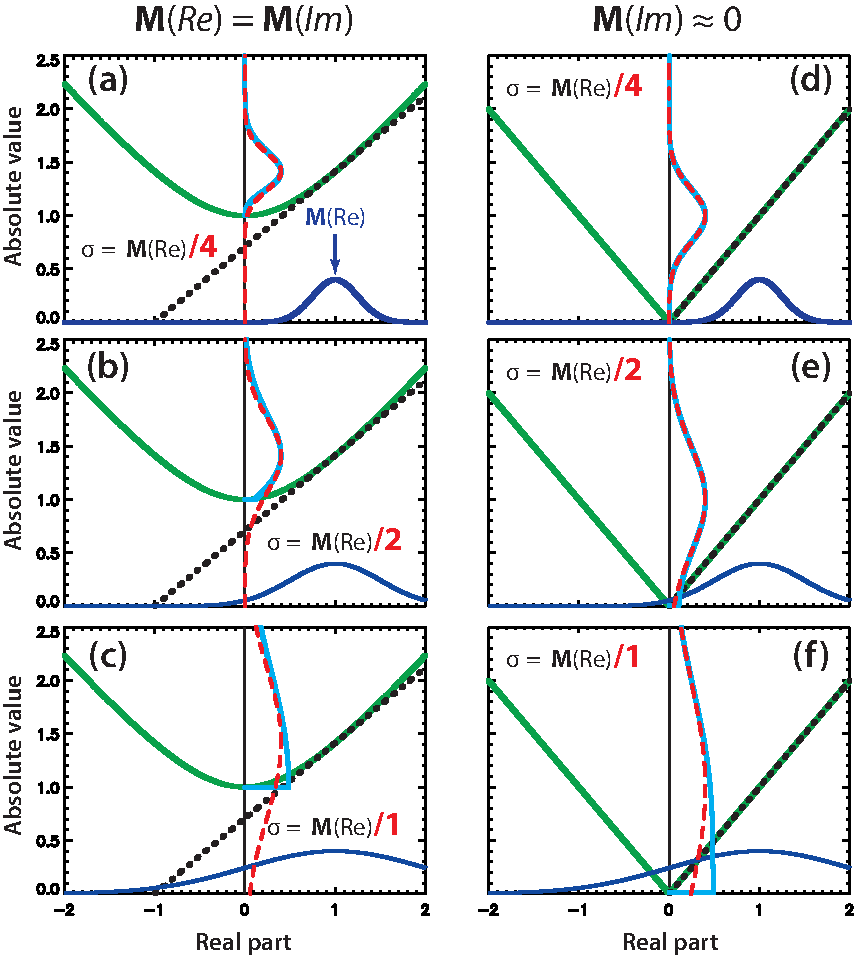
\includegraphics{abs_illustration}}}
  \caption{\label{fig:abs_illustration}Illustration of the error propagation on the absolute value of the Fourier transform. The plots show the distribution of the absolute value calculated by Gauss error propagation (red dashed curves) and the real one (light blue curves) in different cases with different variance of the real part. The imaginary part is fixed.}
\end{figure}
Since this function depends on two variables, we should investigate the problem on a three-dimensional space. For simplicity, the imaginary part is fixed now. The uncertainty of the real part is a Gaussian distribution with $\sigma^2$ variance. On figure \ref{fig:abs_illustration}(a) the dark blue curve shows the shape of the distribution of the real part around the M$(\R)$ expected value. The green curve is the $\Abs(\R,\I)$ function and the light blue curve shows the shape of the distribution of the absolute value, which is the projection of the dark blue curve by the green curve. The black, dotted line is the first derivative of the $\Abs(\R, \I)$ function and the red dashed curve is the distribution arisen from the Gaussian error propagation. This red dashed curve is a Gaussian distribution, since this is the projection of the blue curve, by the black dotted line. So the real distribution of the absolute vale is not a Gaussian, but in this specific case, the two curves (red and light blue) fit well to each other.

Figure \ref{fig:abs_illustration}(b) and \ref{fig:abs_illustration}(c) show a similar case as \ref{fig:abs_illustration}(a), but the variance of the Gaussian distribution is higher so the real distribution (the light cyan curve) is highly biased compared to a Gaussian. As the variance of the real distribution is increasing (respect to the expected value), the bias become larger. Figure \ref{fig:abs_illustration}(d), \ref{fig:abs_illustration}(e) and \ref{fig:abs_illustration}(f) show the case, when the imaginary part is close to zero. If the variance of the real part is not too high (on figure \ref{fig:abs_illustration}(d) and \ref{fig:abs_illustration}(e)) the Gaussian error propagation gives a good approximation. In case, when the variance is higher than the expected value, the Gaussian error propagation is not applicable.

%These figures clearly suggest, that the using of Gauss error propagation will overestimate the uncertainty of the results in all cases. However, in border line cases - like the one on \ref{fig:abs_illustration}(c) - equation \eqref{eq:restriction1} is not satisfied.

To post 5 for the ratio of the first and second terms of equation \eqref{eq:final_exp_abs} as a minimum requirement of using Gauss error propagation is a convenient choice. This is proved in the next section by Monte Carlo methods.

\subsection{Monte Carlo tests}

The presented test was made on a real signal measured by the electron cyclotron emission diagnostics (ECE) of the ASDEX Upgrade tokamak in discharge \#25091. The raw signal and the its energy density - calculated by STFT - is shown in figure \ref{fig:gauss_error_test}(a) and \ref{fig:gauss_error_test}(b) respectively. The $\Delta f(t)$ uncertainty of the $f(t)$ time signal is assumed to be $10\ \%$ of the measured values with Gaussian distribution. First, the uncertainty of the energy density is calculated by the analytical formula introduced in section \ref{sec:ep_analytical}. The results can be seen on figure \ref{fig:gauss_error_test}(c), where the uncertainty in the time-frequency points out of the applicability conditions is set to 0.

The process of the Monte Carlo test is the following. In each $t_i$ time point the $f(t_i)$ measured value has been perturbed by a Gaussian random number with a variance equals to $\Delta f(t_i)$. The energy density of the perturbed signal has been calculated, and this cycle repeated 1000 times. The uncertainty -  which can be seen on figure \ref{fig:gauss_error_test}(d) - in each time-frequency point are given by taking the variance of the spectrograms performed on the perturbed signals.

The agreement of the results (over the region where the applicability condition is satisfied) is clearly seen on figure \ref{fig:gauss_error_test}(c) and \ref{fig:gauss_error_test}(d), but to show it more obviously, the cross-section of the two-dimensional graphs at $t = 2,468$ s can be seen on figure \ref{fig:gauss_error_test}(e) and \ref{fig:gauss_error_test}(f). The previous one shows the cross section of the energy-density, the second one shows the cross-section of the uncertainty. The black dashed line is the result of the Monte Carlo test, the continuous curve is the result of the analytical formula. The red coloured part shows the region, where the applicability condition is satisfied and the light blue part shows the others. The red and the black dashed curve are in a good agreement.

One cross-section of the argument can be seen on figure \ref{fig:gauss_error_test}(g). The uncertainty of it is shown on \ref{fig:gauss_error_test}(h). The results calculated by the analytical formula (red dashed line) and by Monte Carlo method (black solid line) are in good agreement at frequencies where modes with high energy appear.

\begin{figure}[htb!]
  \centerline{\resizebox{120mm}{!}{\includegraphics{gauss_error_test}}}
  \caption{\label{fig:gauss_error_test}The results of the Monte Carlo test: The test was carried out on a real signal (\textit{figure (a)}) measured by the ECE diagnostics of ASDEX Upgrade tokamak. The energy density of the signal is shown on \textit{figure (b)}. The uncertainty of it calculated by the analytical formula (\textit{figure (c)}) and by Monte Carlo method (\textit{figure (d)}) are in good agreement. One cross-section of the energy density (\textit{figure (e)}), the argument (\textit{figure (g)}) and their uncertainty (\textit{figure (f) and (h)}, respectively) are shown.}
\end{figure}



\clearpage

\appendix
\section{The Taylor series for a function that depends on more variables}
A function that depends on more variables, $(x_1,\dots,x_d)$, the Taylor series to second order in the neighbourhood of the point $(a_1,\dots,a_d)$ is:
$$T(x_1,\dots,x_d) = $$
$$=\sum_{n_1=0}^\infty \sum_{n_2=0}^\infty \cdots \sum_{n_d = 0}^\infty 
\frac{(x_1-a_1)^{n_1}\cdots (x_d-a_d)^{n_d}}{n_1!\cdots n_d!}\,\left(\frac{\partial^{n_1 + \cdots + n_d}f}{\partial x_1^{n_1}\cdots \partial x_d^{n_d}}\right)(a_1,\dots,a_d).\!$$

\addcontentsline{toc}{section}{References}
\bibliographystyle{unsrt}
\bibliography{references}

\end{document}